\hypertarget{_benchmark_BenchmarkGraphicsUserInterface}{}\section{Graphics User Interface}\label{_benchmark_BenchmarkGraphicsUserInterface}
The benchmark program should be designed as a G\+U\+I application. Also, it should allow users to configure detail settings such as\+:
\begin{DoxyItemize}
\item Max number of threads
\item Number of objects
\item Methods
\item Duration
\end{DoxyItemize}\hypertarget{_benchmark_BenchmarkMethods}{}\section{Methods}\label{_benchmark_BenchmarkMethods}
The program should has more than one methods to profile the framework. The following algorithm is recommended.
\begin{DoxyItemize}
\item Random objects
\begin{DoxyItemize}
\item Objects appear in random positions
\item Positions change every frame
\end{DoxyItemize}
\item Collision
\begin{DoxyItemize}
\item Objects locate to random position
\item Each object has a random velocity
\item After collision, objects get new velocities
\end{DoxyItemize}
\item Flocking boids
\begin{DoxyItemize}
\item Separation -\/ avoid crowding neighbors
\item Alignment -\/ steer towards average heading of neighbors
\item Cohesion -\/ steer towards average position of neighbors
\end{DoxyItemize}
\end{DoxyItemize}\hypertarget{_benchmark_BenchmarkOutputs}{}\section{Outputs}\label{_benchmark_BenchmarkOutputs}
The output will be a graph which shows all information of the benchmark.
\begin{DoxyItemize}
\item x axis representing number of threads
\item y axis representing frames per second(\+F\+P\+S)
\item values with the maximum, the minimum, and the average.
\end{DoxyItemize}


\begin{DoxyImageNoCaption}
  \mbox{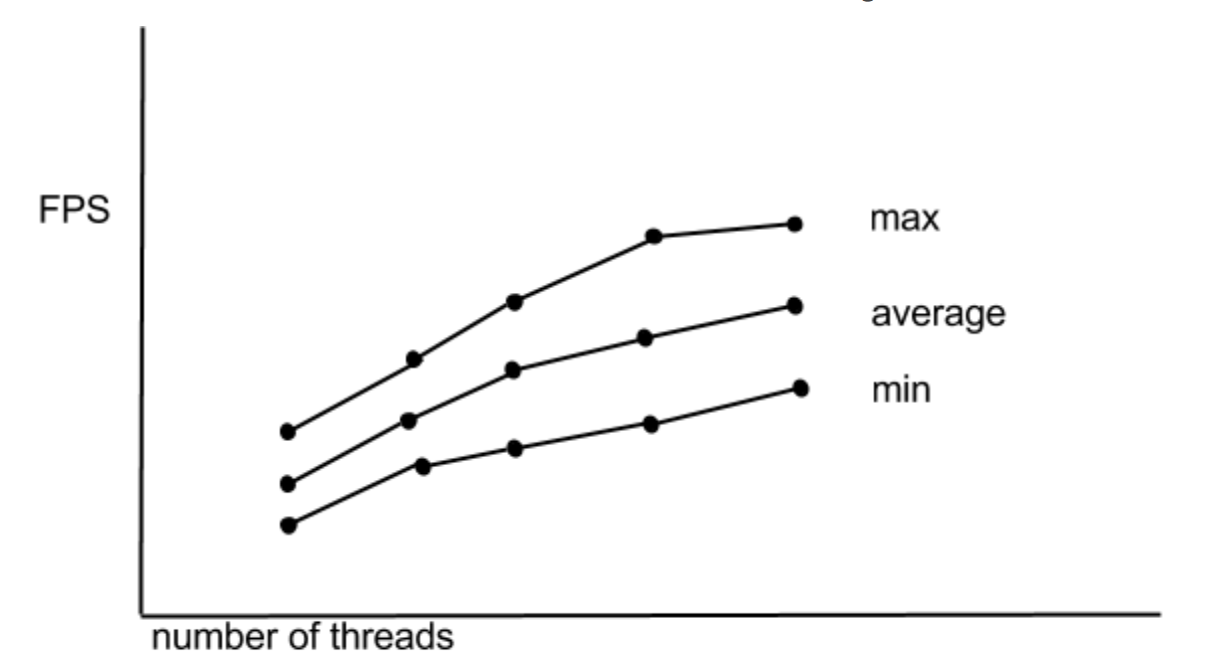
\includegraphics[width=\textwidth,height=\textheight/2,keepaspectratio=true]{FuncSpecOutputs.png}}
\end{DoxyImageNoCaption}
 